\documentclass{article}
\usepackage[margin=1in]{geometry}
\usepackage{amsmath}
\usepackage{amssymb}
\usepackage{graphicx}
\usepackage{tikz}
\graphicspath{images/}

\begin{document}

\title{Golden-Section Search}
\author{Aresh Pourkavoos}
\maketitle

Array $A \in \mathbb{R}^n$
(or any dense totally ordered set) with $n \geq 1$ \\
$A$ attains max at some index $0 \leq i < n$, monotonic on either side, \\
i.e. increasing for indices $\leq i$ and decreasing for indices $\geq i$ \\
All values of $A$ distinct, so strictly monotonic on either side of max,
and elements on opposite sides differ \\
Find $i$ in fewest number of accesses? \\

First, find $A[x]$: max could be anywhere \\
Next, find $A[y]$ for $y \neq x$: WLOG $A[x] < A[y]$ \\
Max is on the side of $A[x]$ containing $A[y]$ \\
Situation is equivalent to where we were before finding $A[y]$,
just with a shorter array and a different index of the known value \\

Problem simplification: given array
and known value at certain position,
determine minimum number of values needed to find max \\
Parameterize situation by sizes of arrays to left and right of known element:
$g(j, k)$ \\
$g(0, 0) = 0$: single element is max \\
$j+k > 0$: consider all options for next split \\
If $j$ split into $j'$ and $k'$ (so $j'+k'+1=j$),
resulting situation is either
$g(j', k')$ (if new element larger) or $g(k', k)$ (if new element smaller) \\
If $k$ split into $j'$ and $k'$ (so $j'+k'+1=k$),
resulting situation is either
$g(j, j')$ (if new element smaller) or $g(j', k')$ (if new element larger) \\
Altogether:
\begin{align*}
  g(j, k) = 1 + \min(
  & \{\max(g(j', k'), g(k', k)) \mid j'+k'+1 = j\} \cup \\
  & \{\max(g(j, j'), g(j', k')) \mid j'+k'+1 = k\})
\end{align*}
\begin{center}
Table of computed values for $j, k < 13$: \\
  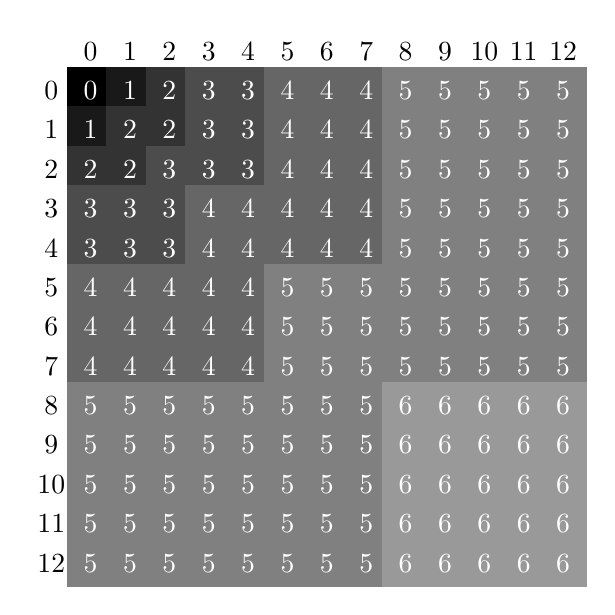
\begin{tikzpicture}[scale=0.5]
    \foreach \y [count=\n from 0] in {
      {0, 1, 2, 3, 3, 4, 4, 4, 5, 5, 5, 5, 5},
      {1, 2, 2, 3, 3, 4, 4, 4, 5, 5, 5, 5, 5},
      {2, 2, 3, 3, 3, 4, 4, 4, 5, 5, 5, 5, 5},
      {3, 3, 3, 4, 4, 4, 4, 4, 5, 5, 5, 5, 5},
      {3, 3, 3, 4, 4, 4, 4, 4, 5, 5, 5, 5, 5},
      {4, 4, 4, 4, 4, 5, 5, 5, 5, 5, 5, 5, 5},
      {4, 4, 4, 4, 4, 5, 5, 5, 5, 5, 5, 5, 5},
      {4, 4, 4, 4, 4, 5, 5, 5, 5, 5, 5, 5, 5},
      {5, 5, 5, 5, 5, 5, 5, 5, 6, 6, 6, 6, 6},
      {5, 5, 5, 5, 5, 5, 5, 5, 6, 6, 6, 6, 6},
      {5, 5, 5, 5, 5, 5, 5, 5, 6, 6, 6, 6, 6},
      {5, 5, 5, 5, 5, 5, 5, 5, 6, 6, 6, 6, 6},
      {5, 5, 5, 5, 5, 5, 5, 5, 6, 6, 6, 6, 6}}
             {
               % labels
               \begin{scope}[shift={(1,0)}]
                 \node[minimum size=6mm] at (\n, 1) {\n};
                 \node[minimum size=6mm] at (-1,-\n) {\n};
               \end{scope}
               % heatmap tiles
               \foreach \x [count=\m, evaluate=\x as \shade using \x*10] in \y {
                 \node[fill=white!\shade!black, minimum size=6mm, text=white] at (\m,-\n) {\x};
               }
             }
  \end{tikzpicture}
\end{center}
Apparent pattern: for all $c \geq 1$,
$g(j, k) < c \iff \min(j, k) < F_c$ and $\max(j, k) < F_{c+1}$ \\
($F_n$ are Fibonacci numbers, $F_0 = 0$, $F_1 = 1$) \\
Proof: \\

$(\impliedby)$ WTS for all $c$,
$\min(j, k) < F_c$ and $\max(j, k) < F_{c+1} \implies g(j, k) < c$ \\
Induct on $c$ \\
Base case $c = 1$: $\min(j, k) < F_1 = 1$ and $\max(j, k) < F_2 = 1$ \\
Then $j = k = 0$, so $g(j, k) = 0 < 1$ \\
Inductive step: suppose $\min(j, k) < F_{c+1}$ and $\max(j, k) < F_{c+2}$,
WTS $g(j, k) < c+1$ \\
If $\max(j, k) = 0$, $j = k = 0$: done \\
Else, can cut $\max(j, k)$ into subsections of size $< F_c$ and $< F_{c+1}$
(since cut itself is $1$ wide) \\
Can place cut so that smaller subsection is adjacent to $\min(j, k)$ \\
Then regardless of whether new cut $>$ old cut,
end up with sections of size $< F_c$ and $< F_{c+1}$ \\
IH: can find max from here in $< c$ steps \\
Thus can find max in $< c+1$ steps \\

$(\implies)$ WTS for all $c$,
$g(j, k) < c \implies \min(j, k) < F_c$ and $\max(j, k) < F_{c+1}$ \\
Contrapositive: $\min(j, k) \geq F_c$ or $\max(j, k) \geq F_{c+1} \implies g(j, k) \geq c$ \\
Induct on $c$ \\
Base case $c = 1$: if $\min(j, k) \geq F_1 = 1$,
then both sections are at least $1$ \\
Thus max cannot be known immediately, so $g(j, k) \geq 1$ \\
If $\max(j, k) \geq F_{c+1}$, then at least one section is $\geq F_2 = 1$,
so as before, $g(j, k) \geq 1$ \\
Inductive step: suppose $\min(j, k) \geq F_{c+1}$ or $\max(j, k) \geq F_{c+2}$,
WTS $g(j, k) \geq c+1$ \\
If $\min(j, k) \geq F_{c+1}$, then both sections are $\geq F_{c+1}$ \\
Then regardless of which section is cut, the other could remain \\
Thus max of new sections could be $\geq F_{c+1}$,
so by IH, could require $\geq c$ more cuts in the worst case \\
Thus $\geq c+1$ cuts required overall \\
If $\max(j, k) \geq F_{c+2}$,
first suppose $\min(j, k)$ is cut \\
Then the max might not change,
as the new value could be $<$ the known one \\
Then new max is $\geq F_{c+2} \geq F_{c+1}$,
so by IH, $\geq c$ more cuts required in the worst case \\
Thus $\geq c+1$ cuts required overall \\
Now suppose instead $\max(j, k)$ is cut \\
New value could be $>$ known one: assume it is in the worst case,
so sum of new subsections is $F_{c+2}-1$ \\
$F_{c+2} = F_c+F_{c+1}$ and $F_c \geq F_{c+1}$,
so either min $\geq F_c$ or max $\geq F_{c+1}$
(even with loss of $1$ in cut itself) \\
By IH, $\geq c$ more cuts required, so $\geq c+1$ cuts required overall \\

Directions of proof provide strategies for ``opponents'' in search ``game'' \\
$(\impliedby)$ gives strategy for searcher, which implements golden-section search \\
$(\implies)$ gives adversarial input with worst-case performance \\

Very start of search: no elements known \\
If starting length is $1$, know max with $0$ steps \\
Else, must choose initial cut that minimizes remaining number of steps \\
If $n < F_{c+2}-1$, can choose cut with min $< F_c$ and max $< F_{c+1}$ \\
Thus, can find max in $< c$ more steps, so $< c+1$ total \\
Else, cannot choose such a cut, so $\geq c$ steps needed in the worst case
for $\geq c+1$ total \\
So worst-case cost for length $n$ is
$0$ if $n = 1$ and smallest $c$ such that $n < F_{c+2}-1$ otherwise \\

Slight relaxation of problem: 
elements on opposite sides of max may be the same,
but 

\end{document}
